%!TEX root = ../TTK4550-MHT.tex
\section{Linear programming}
\label{sec:ilp}
The aim of this section is to elaborate the use of linear programming to solve the data association problem in MHT that arises when there are multiple (possible mutual exclusive) possibilities of measurement arrangements within the existing set of tracks. As with any optimization problem, we need an objective function which tells us how good or bad a given assignment is, and a set of constraints that limits the solution to the physical limits and our assumptions.

\subsection{Problem formulation}
Storms and Spieksma \cite{Storms2003} are suggesting an Integer Linear Programming (ILP) scheme with Linear Programming (LP) relaxation and Greedy Rounding Procedure (GRP) as solvers. 
\begin{equation}
\begin{aligned}
& \underset{f}{\text{minimize}}
& & f=\sum_{z \in \V{Z^*}} c_z x_z \\
& \text{subject to}
& & \sum_{z \in \V{Z^*} , z(k)=z_{i_k}^k} x_z=1 , \forall k = 1, \ldots, N   \text{ and } i_k = 1, \ldots, M_k  \\
&&& x_z \in \{0,1\}
\end{aligned}
\end{equation}
where, $c_z = -lnQ_z$ and the likelihood for a track is
\begin{equation}
Q(z) = \prod_{k=1}^N (P_\phi^k)^{\Delta_{i_k}} \left \{ 
	\left[ \frac{P_d f_\delta^k (z_{i_k}^k | z)}{\lambda_\varphi f_\varphi^k(z_{i_k}^k)} \right]^{\delta_{i_k}^k} 	
	\left[ \frac{\lambda_\nu f_\nu^k(z_{i_k}^k|z)}{\lambda_\varphi f_\varphi^k(z_{i_k}^k)} \right]^{\nu_{i_k}^k}
	\right \}^{(1-\Delta_{i_k})}
\end{equation}
where,
\begin{equation*}
\begin{split}
	\Delta_{i_k} 	&= 
		\begin{cases} 
			1, i_k=0 (\text{dummy-report}) \\ 
			0, \text{otherwise} 
		\end{cases} \\
	P_\phi^k 		&=
		\begin{cases} 
			1-P_d, z_{i_k}^k \text{is a missing report} \\ 
			0, \text{otherwise} 
		\end{cases} \\
	\nu_{i_k}^k 	&=
		\begin{cases} 
			1, z_{i_k}^k \text{initiates a track} \\ 
			0, \text{otherwise} 
		\end{cases} \\
	\delta_{i_k}^k 	&=
		\begin{cases} 
			1, z_{i_k}^k \text{proceeds as a track} \\ 
			0, \text{otherwise} 
		\end{cases} \\
	P_d 			&= \text{probability of detection} \\
	\lambda_\varphi &= \text{expected number of false alarms (Poisson distribution)} \\
	\lambda_\nu		&= \text{expected number of new targets (Poisson distribution)} \\
	f_\nu^k 		&= f_\varphi^k = \frac{1}{\pi r^2}, \text{where r is the sensor range} \\
	f_\delta^k 		&= \frac{e^{-\frac{1}{2}[z_{i_k}^k-h(\bar{s}(t_k))]^T B^{-1} [z_{i_k}-h(\bar{s}(t_k))] }}{\sqrt{(2\pi)^n |B|}} \\
	n 				&= \text{dimension of measurement vector} \\
	h(\cdot)		&= \text{transformation of Cartesian to polar} \\
	\bar{s}			&= \text{predicted state vector} \\
	B 				&= \text{covariance of } z_{i_k}^k - h(\bar{s}(t_k))
\end{split}
\end{equation*}
This approach uses a rather inelegant summation notation which is not on a standard (I)LP format. 

In this work we propose a more compact formulation of the data association problem on ILP standard form.
\begin{equation}
\begin{aligned}
&	\underset{}{\text{maximize}}
&&	\V{c}^T \V{x} \\
&	\text{s.t.}
&&	\M{A_1} \V{x} \leq \V{b_1} 	\\
&&&	\M{A_2} \V{x} = \V{b_2}	\\
&&&	\V{x} \in \{0,1\}
\end{aligned}
\end{equation}
Where $\M{A_1}$ is a $N_1 \times M$ binary matrix with $N_1$ real measurements and $M$ track hypotheses (all leaf nodes), where $\M{A_1}(i,j)=1$ if hypothesis $j$ are utilizing measurement $i$, $0$ otherwise. The measurements and hypothesis are indexed by the order they are visited by a depth first search (DFS). $\M{A_2}$ is a $N_2 \times M$ binary matrix where $N_2$ is the number of targets in the cluster and $\M{A_2}(i,j)=1$ if hypothesis $j$ belongs to target $i$. $\V{b_1}$ is a $N_1$ long vector with ones and $\V{b_2}$ is a $N_2$ long vector with ones. $\V{c}$ is a $N$ long vector with a measure of the goodness of the track hypotheses. For example in Figure \ref{fig:hyp-tree} at time step 2, the A matrices  and C vector would be:
\begin{equation}
\begin{split}
\M{A_1} &=\begin{bmatrix}
		0 & 1 & 1 & 0 & 0 & 0 & 0 & 0 & 0 \\
       	0 & 0 & 1 & 0 & 0 & 1 & 0 & 1 & 0 \\
       	0 & 0 & 0 & 1 & 0 & 0 & 1 & 1 & 1 \\
       	0 & 0 & 0 & 0 & 0 & 0 & 0 & 0 & 1 \\
     	\end{bmatrix}
\V{b_1} = 	\begin{bmatrix}
			1 \\ 1  \\ 1 \\ 1
			\end{bmatrix} \\
\M{A_2} &=\begin{bmatrix}
		1 & 1 & 1 & 1 & 0 & 0 & 0 & 0 & 0 \\
       	0 & 0 & 0 & 0 & 1 & 1 & 1 & 1 & 1 \\
     	\end{bmatrix} 
\V{b_2} = 	\begin{bmatrix}
			1 \\ 1
			\end{bmatrix} \\
\V{c} &=\begin{bmatrix}
		\lambda_1 & \lambda_2 & \lambda_3 & \lambda_4 & \lambda_5 & \lambda_6 & \lambda_7 & \lambda_8 & \lambda_9
		\end{bmatrix}^T \\
\end{split}
\end{equation}

\begin{figure}
\centering
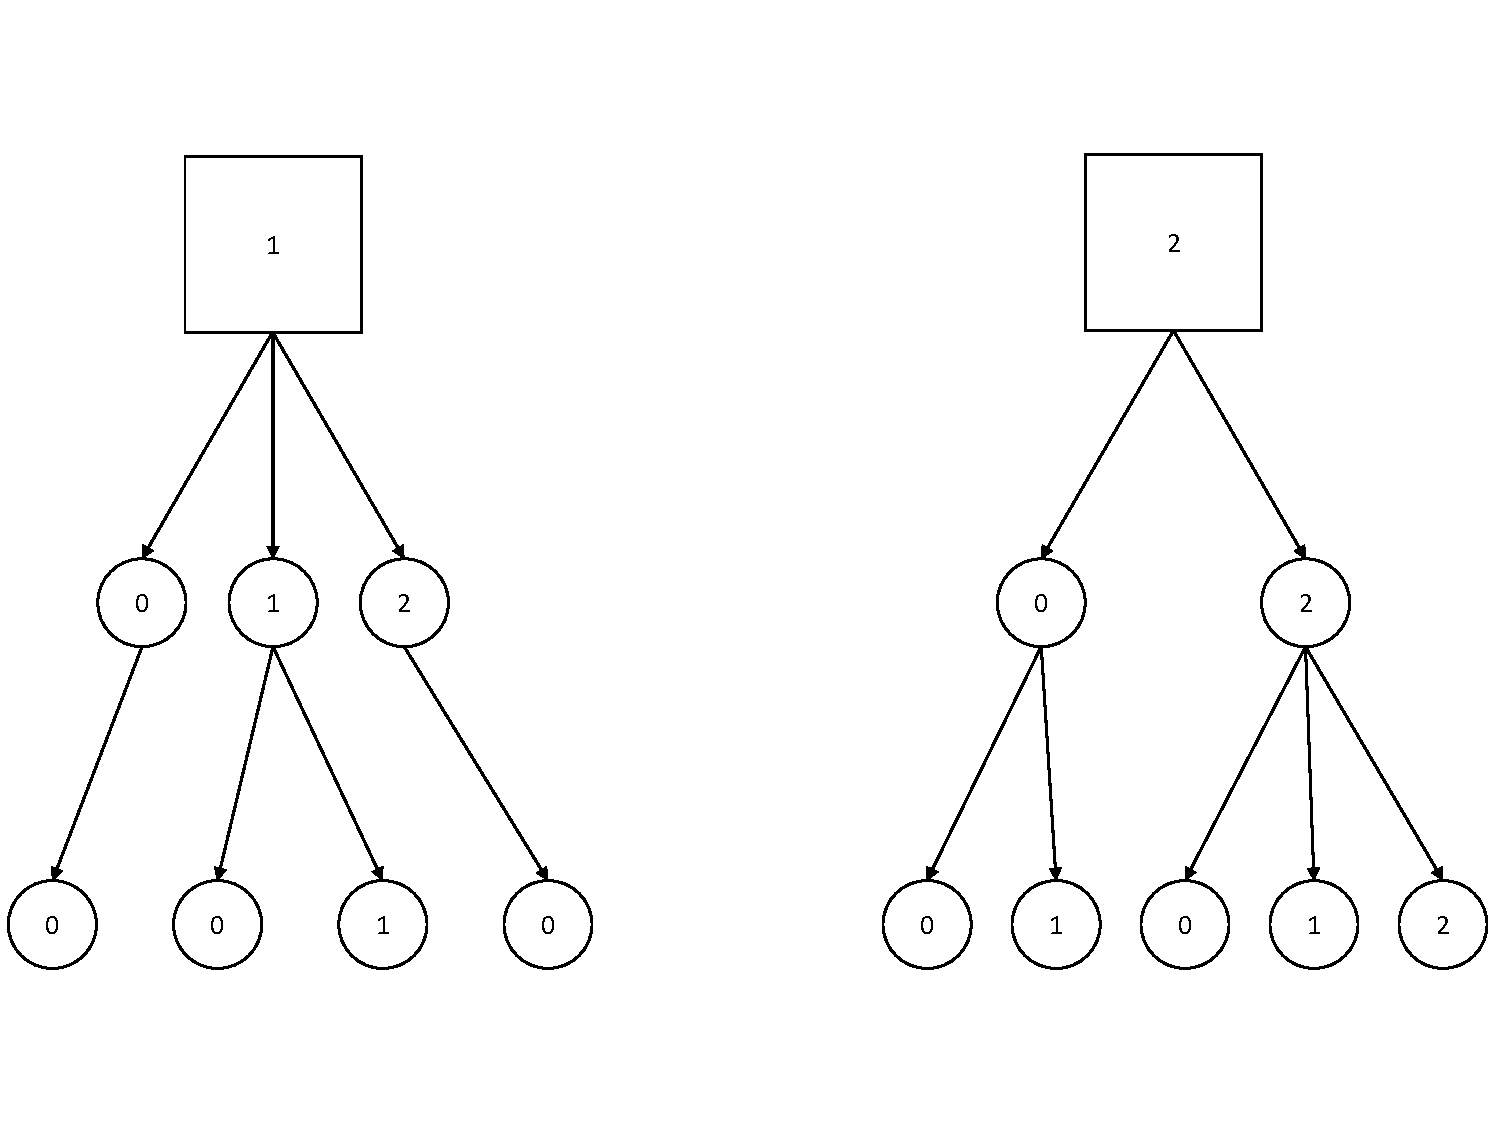
\includegraphics[width = .8\textwidth]{Track-tree}
\caption{Track hypothesis tree}
\label{fig:hyp-tree}
\end{figure}

\subsection{Solvers}
There are a lot of of-the-shelf integer linear program (ILP) and mixed integer linear program (MILP) solvers on the marked, both free open source and commercial. Since our problem is formulated on standard form, it can easily be executed on several solvers, and we can compare runtime and performance. In this report, the following solver are tested:
\begin{itemize}
\item CPLEX 	(Commercial (Free academic),  IBM)
\item GLPK 		(Free, GNU)
\item CBC 		(Free, COIN-OR)
\item SYMPHONY	(Free, COIN-OR)
\item Gurobi 	(Commercial (Free academic), Gurobi)
\item Xpress	(Commercial, FICO)
\end{itemize}

















